%%%%%%%%%%%%%%%%%%%%%%%%%%%%%%%%%%%%%%%%%%%%%%%%%%%%
%												   %
%	ESCOLA   									   %
%												   %
%	Marco 2015  								   %
%												   %
%	Angela Cardoso, Rui Costa e Ricardo Lopes	   %
%   											   %	
%%%%%%%%%%%%%%%%%%%%%%%%%%%%%%%%%%%%%%%%%%%%%%%%%%%%

\documentclass[12pt,a4paper,reqno]{report}
\linespread{1.5}

\usepackage{amsfonts,amsmath,amssymb,indentfirst,mathrsfs,amscd}
\usepackage[mathscr]{eucal}
\usepackage[active]{srcltx} %inverse search
\usepackage{tensor}
\usepackage[utf8x]{inputenc}
\usepackage[portuges]{babel}
\usepackage[T1]{fontenc}
\usepackage{tikz}
\usepackage{graphicx}
\usepackage[numbers,square, comma, sort&compress]{natbib}
\numberwithin{figure}{section}
\numberwithin{equation}{section}
\usepackage{scalefnt}
\usepackage[top=2.5cm, bottom=2.5cm, left=2.5cm, right=2.5cm]{geometry}
\usepackage{comment} 
%\usepackage{tweaklist}
%\renewcommand{\itemhook}{\setlength{\topsep}{0pt}%
%	\setlength{\itemsep}{0pt}}
%\renewcommand{\enumhook}{\setlength{\topsep}{0pt}%
%	\setlength{\itemsep}{0pt}}
%\usepackage[colorlinks]{hyperref}
\usepackage{MnSymbol}
%\usepackage[pdfpagelabels,pagebackref,hypertexnames=true,plainpages=false,naturalnames]{hyperref}
\usepackage[naturalnames]{hyperref}
\usepackage{enumitem}
\usepackage{titling}
\newcommand{\subtitle}[1]{%
  \posttitle{%
    \par\end{center}
    \begin{center}\large#1\end{center}
    \vskip0.5em}%
}
\newcommand{\HRule}{\rule{\linewidth}{0.5mm}}

\usepackage[official]{eurosym}

\def\Cpp{C\raisebox{0.5ex}{\tiny\textbf{++}}}

\makeatletter
\def\@makechapterhead#1{%
  %%%%\vspace*{50\p@}% %%% removed!
  {\parindent \z@ \raggedright \normalfont
    \ifnum \c@secnumdepth >\m@ne
        \huge\bfseries \@chapapp\space \thechapter
        \par\nobreak
        \vskip 20\p@
    \fi
    \interlinepenalty\@M
    \Huge \bfseries #1\par\nobreak
    \vskip 40\p@
  }}
\def\@makeschapterhead#1{%
  %%%%%\vspace*{50\p@}% %%% removed!
  {\parindent \z@ \raggedright
    \normalfont
    \interlinepenalty\@M
    \Huge \bfseries  #1\par\nobreak
    \vskip 40\p@
  }}
\makeatother


\begin{document}



\begin{titlepage}
\begin{center}
 
\vspace*{3cm}

{\Large Bases de Dados}\\[1.5cm]

% Title
{\Huge \bfseries Escola Secundária \\[2cm]}

% Author
{\large Ângela Cardoso, Rui Costa e Ricardo Lopes}\\[2cm]


\includegraphics[width=10cm]{feup_logo.jpg}\\[2cm]


% Bottom of the page
{\large \today}

\end{center}
\end{titlepage}

\tableofcontents

%%%%%%%%%%%%%%
% INTRODUCAO %
%%%%%%%%%%%%%%
\chapter{Introdução}

No âmbito da unidade curricular Bases de Dados, do Mestrado Integrado em Engenharia Informática e Computação, decidimos modelar e implementar uma base de dados para gestão de uma escola secundária.

O sistema deve conter informação sobre alunos, docentes, encarregados de educação, disciplinas, turmas e áreas, permitindo a adição de novos elementos, assim como a consulta dos elementos previamente adicionados e das relações existentes entre eles.

Ao longo deste documento descreve-se o modelo UML que desenvolvemos para a referida base de dados. Em particular, são explicadas as várias restrições consideradas, o tipo de situações que estão enquadradas neste modelo, assim como aquelas que estão fora do âmbito da solução que propomos.

%%%%%%%%%%%%%
% DESCRICAO %
%%%%%%%%%%%%%
\chapter{Descrição do Contexto}

Numa escola secundária há 3 grupos de pessoas fundamentais: os professores, os alunos e os encarregados de educação. Cada um destes grupos tem um papel distinto, com o objetivo comum de formar os alunos no âmbito das respetivas áreas escolhidas. Além destas pessoas, numa escola também podemos encontrar funcionários e diretores. No entanto, como veremos mais adiante, estes não são contemplados no modelo que construímos.

Além de algumas tarefas de estilo mais administrativo, como reuniões ou elaboração de relatórios, as principais responsabilidades dos professores são dar aulas e avaliar os alunos. Um professor que seja diretor de turma, tem ainda que reunir com os encarregados de educação dos alunos dessa turma, consoante as necessidades do aluno.

Os alunos têm como principais tarefas a frequência das aulas, o estudo fora destas e a realização das diversas provas de avaliação.

O encarregado de educação deve acompanhar o aluno nos seus estudos e reunir com o diretor de turma, para ajudar a optimizar o aproveitamento do aluno.

Os alunos estão organizados em turmas, consoante o ano que frequentam, e a área dos seus estudos. Para cada turma há um professor responsável (o diretor de turma), um conjunto de disciplinas e um professor responsável por cada disciplina.

A escola providencia várias áreas de formação, consoante o ramo e o tipo de curso. Por exemplo, no ramo científico poderá haver áreas de carácter geral e de caráter tecnológico ou mesmo profissional. Para cada área de formação existe um professor responsável.

Um ano letivo é constituído por um ou mais períodos de avaliação. Atualmente, o ano letivo está dividido em 3 períodos, mas é possível que isso seja alterado no futuro. Em cada período os alunos são avaliados nas disciplinas que frequentam obtendo uma classificação que fica registada.

%%%%%%%%%%%%%
% DESCRICAO %
%%%%%%%%%%%%%
\chapter{Descrição da Solução Implementada}

No modelo desenvolvido, consideramos as seguintes classes principais:
\begin{itemize}
\item \textbf{Pessoa} - superclasse que contém a informação comum aos docentes, alunos e encarregados de educação, como o número de identificação na escola, o nome, a morada, a data de nascimento, etc;
\item \textbf{Docente} - tem atributos próprios, como o ano de admissão e as qualificações;
\item \textbf{Aluno} - tal como o docente, tem um ano de entrada na escola, tendo ainda um campo de observações, como por exemplo uma suspensão ou uma condição médica que seja do interesse da escola;
\item \textbf{Encarregado\_Educação} - tem um horário preferencial para ser contactado pela escola, sendo esse contacto normalmente efetuado pelo diretor de turma de um dos alunos pelo qual é responsável;
\item \textbf{Área} - contém informação sobre o tipo de curso, nomeadamente, se se trata de um curso de carácter geral, tecnológico ou profissional, assim como o ramo a que pertence;
\item \textbf{Turma} - é identificada por um número e pelo ano escolar a que pertence, além disso está associada a um ano letivo específico;
\item \textbf{Disciplina} - possui um código de identificação da escola, assim como o nome e a descrição;
\item \textbf{Ano\_Letivo} - tem uma data de início e uma data de fim, sendo constituído por vários períodos letivos;
\item \textbf{Período} - é identificado por um número, contendo ainda informação sobre as datas em que inicia e termina.
\end{itemize}

Além destas, abstraímos também os conceitos de \textbf{Código\_Postal} e \textbf{Localidade}, tendo surgido ainda classes de relação entre algumas das classes vistas no ponto anterior, que descreveremos mais adiante.

Para cada par turma e disciplina, existe um único professor associado. No entanto, um dado professor pode estar apto a lecionar outras disciplinas além destas, estando essa informação contida na base de dados da escola. Há ainda uma relação entre cada turma e um docente específico: o diretor de turma. Uma dada turma tem um e um só diretor, que à partida será responsável pela turma durante todo o ano letivo. No entanto, em situações excepcionais, poderá ser necessária a substituição do diretor de turma, sendo isso contemplado no modelo que desenhamos.

Os alunos são classificados a todas as disciplinas que frequentam consoante o período do ano letivo. As disciplinas frequentadas por um dado aluno são determinadas consoante a turma em que ele está inserido. Sendo que a turma, por sua vez, depende do ano escolar e da área de formação dos seus alunos.

À semelhança daquilo que acontece com os diretores de turma, cada área possui um único responsável em cada momento. No entanto, esse responsável poderá variar ao longo do tempo. Em princípio, um dado docente não é responsável por mais do que uma área ao mesmo tempo.

Os encarregados de educação e os diretores de turma podem marcar reuniões por iniciativa de qualquer um deles, ficando registadas a data, a hora e a sala da reunião. Excepcionalmente, um encarregado de educação poderá reunir com outro professor do aluno pelo qual é responsável, ficando essa reunião registada da mesma forma. Cada aluno possui um único encarregado de educação (que pode ser responsável por vários alunos), sendo registada a relação de parentesco do encarregado com o aluno. Em alguns casos essa relação poderá não ser familiar, no entanto é sempre usada a palavra parentesco, ainda que no sentido lato.

Consideramos que é possível uma mesma pessoa ser simultaneamente docente da escola e encarregado de educação. Além disso, embora apenas em casos muitos especiais, um determinado aluno pode ser também encarregado de educação (de si próprio ou de outro aluno), nomeadamente se esse aluno for maior de idade ou tiver sido emancipado.

No modelo que desenhamos, não são contemplados os horários das várias aulas. Sendo assim, não é possível determinar o horário de um determinado aluno ou de um professor. Também não é incluída qualquer informação sobre os funcionários da escola, sobre os seus diretores ou sobre eventuais enfermeiros ou psicólogos. Numa versão mais alargada, poderiam e deveriam ser consideradas estas classes. Também seria interessante considerar informação mais detalhada sobre o percurso do aluno na escola, como por exemplo alterações significativas na sua vida pessoal, registos de faltas, visitas à enfermagem ou ao gabinete de psicologia, testes psicotécnicos que tenha efetuado, projetos e grupos extracurriculares em que tenha estado envolvido, etc.

%%%%%%%%%%%%
% DIAGRAMA %
%%%%%%%%%%%%
\chapter{Diagrama de Classes UML}

\begin{center}

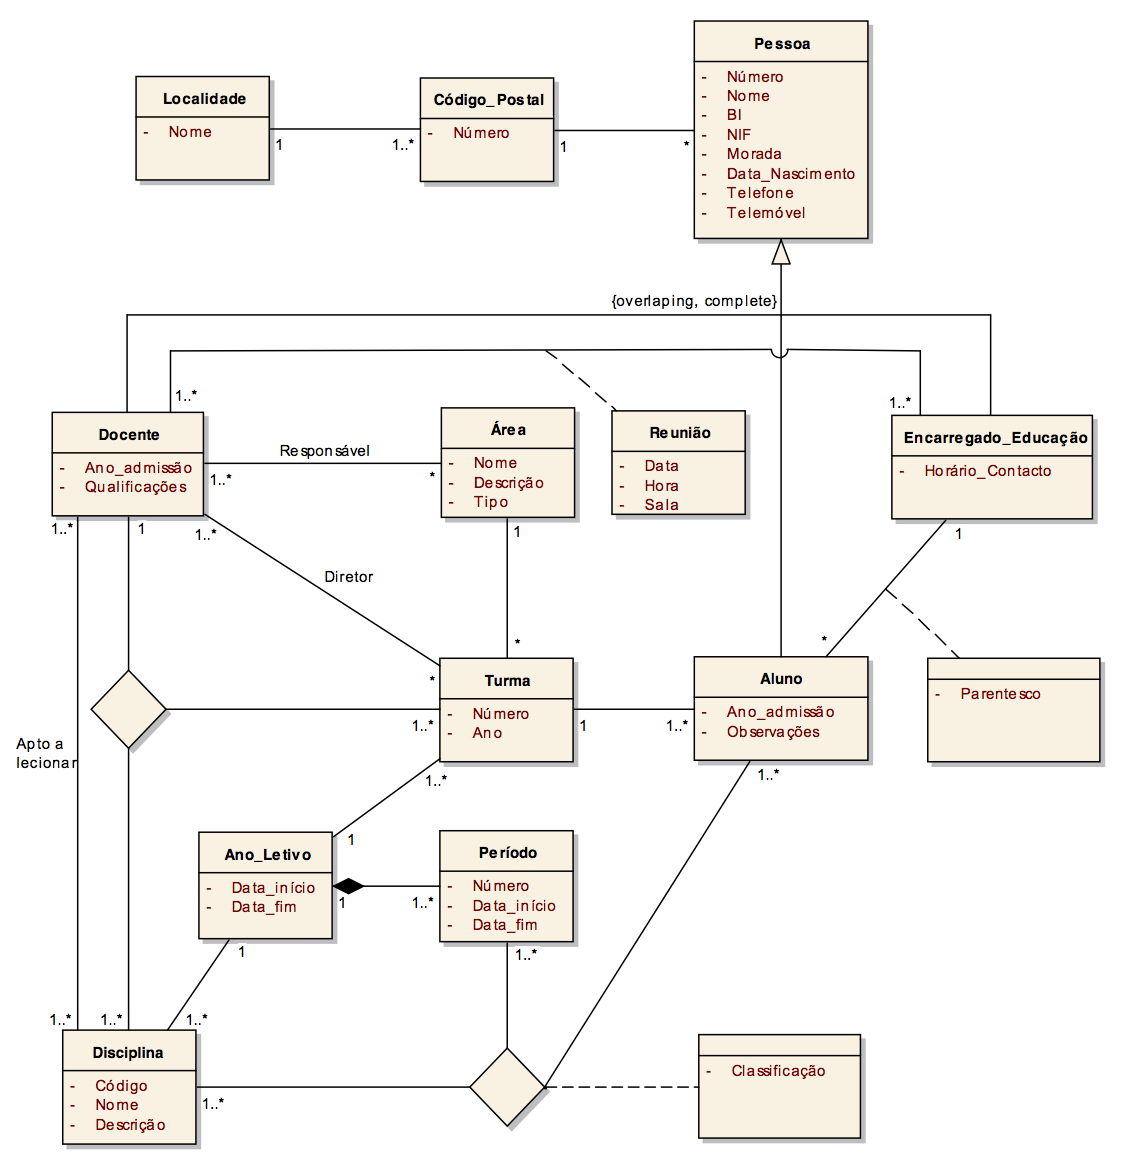
\includegraphics[width=15cm]{UML.jpg}

\end{center}

%%%%%%%%%%%%%%%%
% DIFICULDADES %
%%%%%%%%%%%%%%%%
\chapter{Principais Dificuldades}

Essencialmente surgiram dificuldades na escolha das relações apropriadas entre as várias classes, assim como da multiplicidade dessas relações. Por exemplo, os casos em que num momento específico existe um único elemento, mas ao longo do tempo podem existir vários não foram inicialmente bem identificados.

A escolha das situações que seriam excluídas do modelo elaborado também suscitou algumas dúvidas. No final, acabamos por decidir em função do nível de complexidade pretendido para este projeto, tentando não obter um modelo demasiado extenso.

Finalmente, a comunicação entre os elementos do grupo fora do horário das aulas também levantou alguns problemas. Embora praticamente todo o trabalho de concepção e desenho do modelo de classes tenha sido efetuado em conjunto por todos os elementos, tal não foi possível na parte final do trabalho, nomeadamente na elaboração do presente relatório.

%%%%%%%%%%%%%
% CONCLUSAO %
%%%%%%%%%%%%%
\chapter{Conclusão}

Apesar de considerarmos que o modelo escolhido contempla uma boa variedade de situações, no que diz respeito à informação útil para uma escola secundária, teria sido interessante incluir mais situações, se a duração do projeto assim o permitisse. De facto, numa fase inicial do projeto pensamos que seria possível considerar mais classes. Só ao elaborar o diagrama UML nos apercebemos da verdadeira complexidade do problema.

O trabalho em si está a ser muito interessante, especialmente pela possibilidade de aplicar uma grande parte dos conceitos que foram introduzidos na unidade curricular, tornando-se mais fácil a sedimentação desses mesmos conceitos. Também foi particularmente curioso verificar num caso concreto o quanto este tipo de trabalho é subjetivo, sendo possível para um mesmo tema obter modelos muito diferentes.

\end{document}
